
\section{The Data Set}
For the following we us a data set generated by 
%
\begin{changemargin}{1.5cm}{1.5cm} 
  \lstinputlisting[numbers=left,firstnumber=1,firstline=1]{../examples/core/data/produce_data.py}
\end{changemargin}
%
As can be seen, there is one gaussian blob located at zero. The other
data set, considered as signal in the following is made up from two
gaussians.

\section{Plotter}
With the following puthon snippet we produce two gaussian
distributions of some pseudo data. We then plot the scatter in the x,y
plane as well as histograms for the x and y axis.
%
\begin{changemargin}{1.5cm}{1.5cm} 
  \lstinputlisting[numbers=left,firstnumber=1,firstline=1]{../examples/core/plotter/example.py}
\end{changemargin}
%
%
\begin{figure}
  \centering
  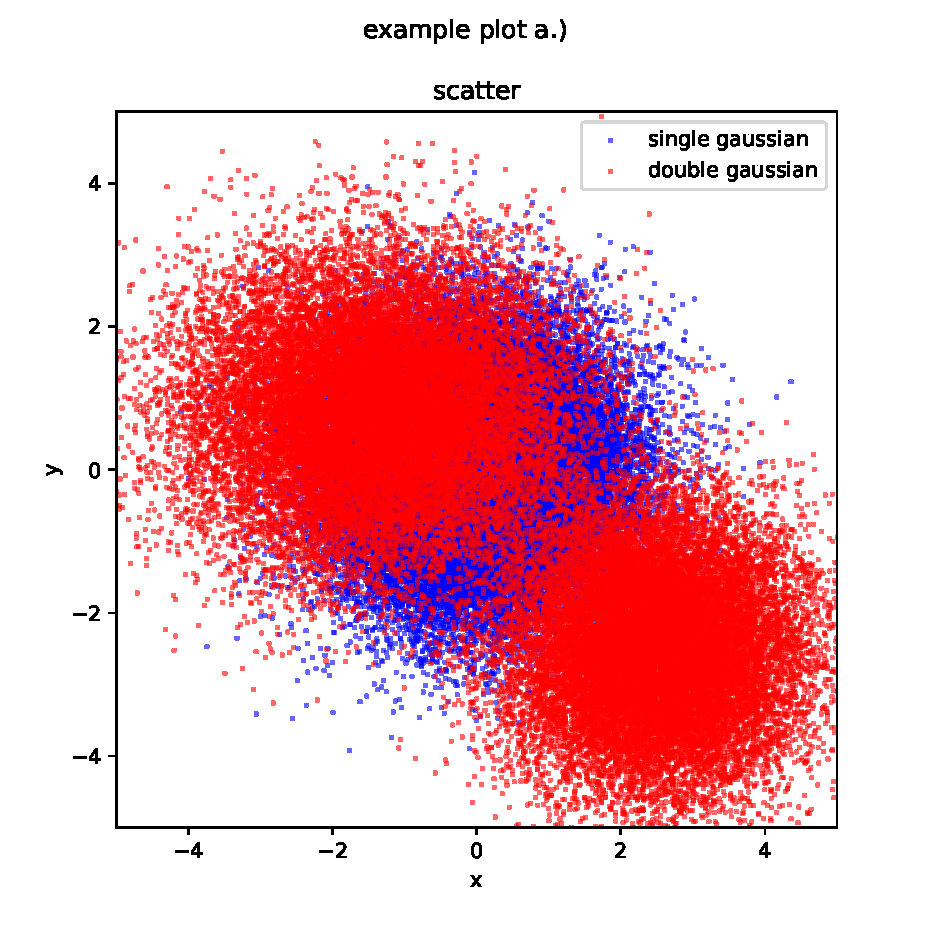
\includegraphics[width=0.32\textwidth]{../examples/core/plotter/example_a.pdf}
  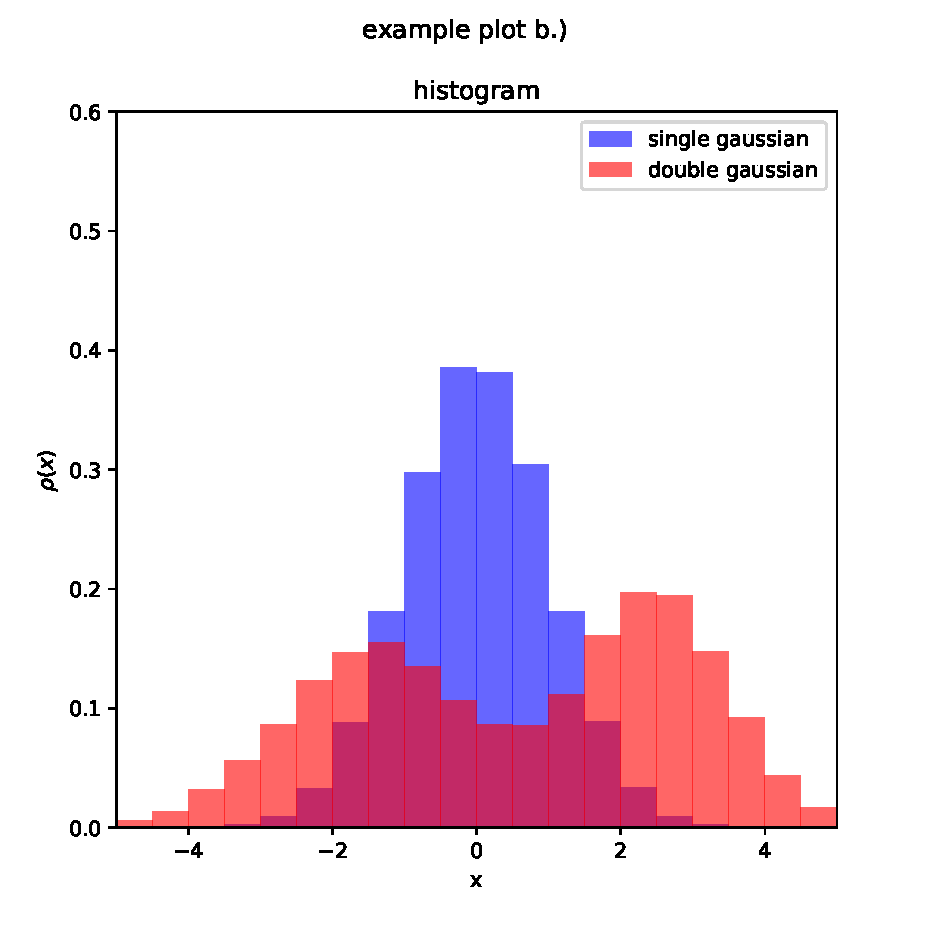
\includegraphics[width=0.32\textwidth]{../examples/core/plotter/example_b.pdf}
  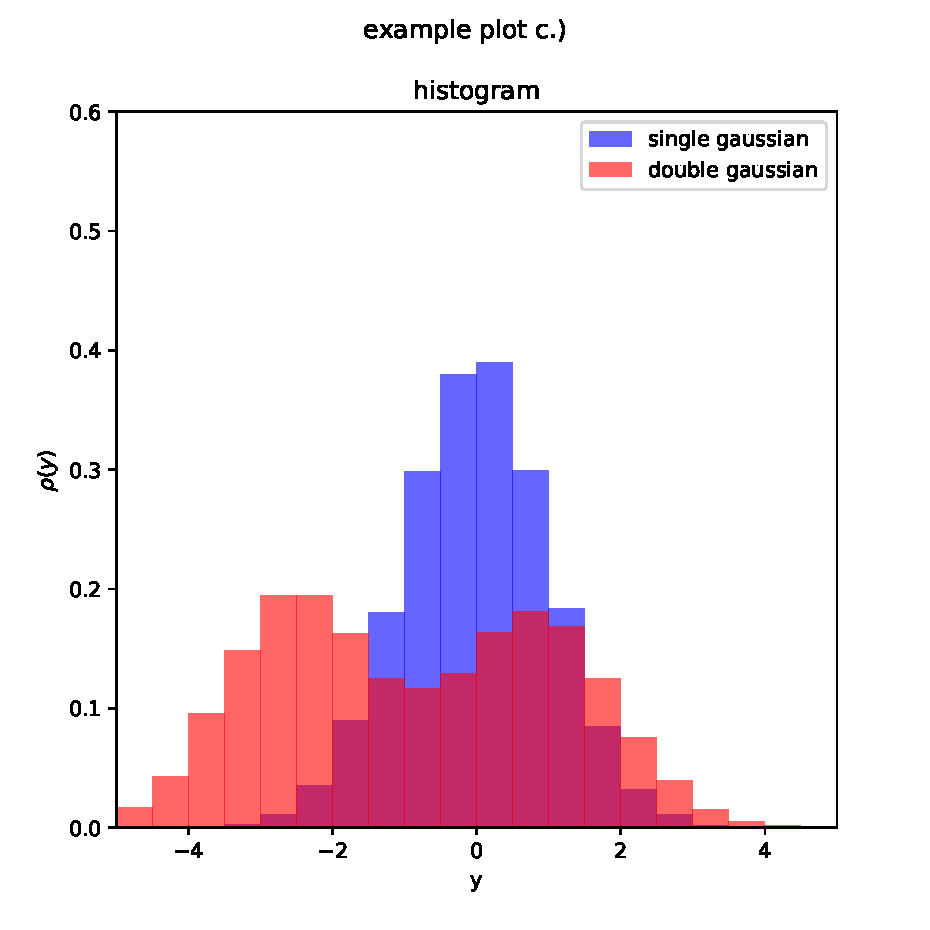
\includegraphics[width=0.32\textwidth]{../examples/core/plotter/example_c.pdf}
  \caption{}
  \label{fig:example_plotting}
\end{figure}
%
In Fig.~\ref{fig:example_plotting} we present the result. Note, that
the same results can be obtained when instead invoking hepstore-plot
from the command line.

